\chapter{Image compressive sensing}
\label{chap:image-cs}


One of the more intuitive applications of CS lies in spatial signals as it is easier to visualize. In this scheme, the process can be simplified either by flattening it to one dimension and processing it in its entirety, or maintaining its dimensionality and processing it by patches. The general workflow that arises from image CS is as follows:

\begin{enumerate}
	\item Define the compression ratio $m/n$, where $n$ is the signal size, and $m$ is the desired size of the compressed signal.
	\item Draw $m$ random indices from the signal without replacement and store this as a sample sequence $\bm\xi$.
	\item Extract the row vectors of the desired $n \times n$ sparsifying basis $\bm\Psi$ indexed by $\bm\xi$, and stack these to form the sensing matrix $\bm\Phi$ (i.e., $\bm\Phi = \bm\Psi_{\bm\xi}$)
	\item With the desired reconstruction algorithm, perform the optimization \eqref{eq:min-l1} to obtain the reconstructed signal $\bm\hat{\vec{x}}$.
\end{enumerate}

In the case of high-definition images (whose shortest side is at least 720 pixels), it is usually more practical and yields better results if the image is processed in patches.


\section{Test case: Sinusoidal pattern}
\label{sec:2dsin}
As mentioned in Chapter~\ref{chap:theory}, the most commonly used sparse representation domain for images is the Fourier domain, referred to in some fields as $k$-space. In this space, signals are represented as a linear superposition of a finite number of sinusoidal patterns. In Fig.~\ref{fig:2dsin}, $64 \times 64$ pixel sinusoidal patterns are generated, corresponding to sine waves traveling horizontally, vertically, and diagonally, as well as an egg tray pattern. In each case, all frequency components are 4 Hz. Figure~\ref{fig:2dsin-masked} visualizes the compressed image when a random sample of 5\% is taken from the signal. The actual compressed signal that is seen by the reconstruction algorithm is a one-dimensional sequence containing only the information from the points being sampled. Orthogonal matching pursuit (OMP) was used for reconstruction, which is a greedy algorithm that finds the combination of basis vectors which best represents the signal (similar to matching pursuit), but in addition, the residual at each iteration is recomputed using an orthogonal projection on the set of previously selected basis vectors \cite{Mallat1993}. Its objective function is

\begin{equation}\label{eq:omp}
	\arg\min_{\vec{x}} \norm{\vec{y} - \bm\Phi \vec{x}}_2^2 \quad \textrm{subject to} \quad \norm{\vec{x}}_0 \leq \gamma
\end{equation}

\noindent where $\gamma$ is a hyperparameter which controls the maximum allowable number of non-zero coefficients. The \texttt{Scikit-learn} implementation sets this value to 10\% of the number of samples by default \cite{scikit-learn}. Evaluation of the mean-squared error (MSE) for the pure horizontal and pure vertical sine waves, as well as the egg tray pattern yields a value that is practically negligible ($\approx 10^{-31}$); the reconstruction is exact. On the other hand, the reconstructed diagonal sine wave yields an MSE of $10^{-3}$---still quite small, but mild distortion can be observed at the image boundaries. This is due to the fact that the information at hand is finite, and so is the window size which, in this case, is the same size as the signal itself.

\begin{figure}[htb]
	\centering
	\begin{subfigure}{\textwidth}
		\centering
		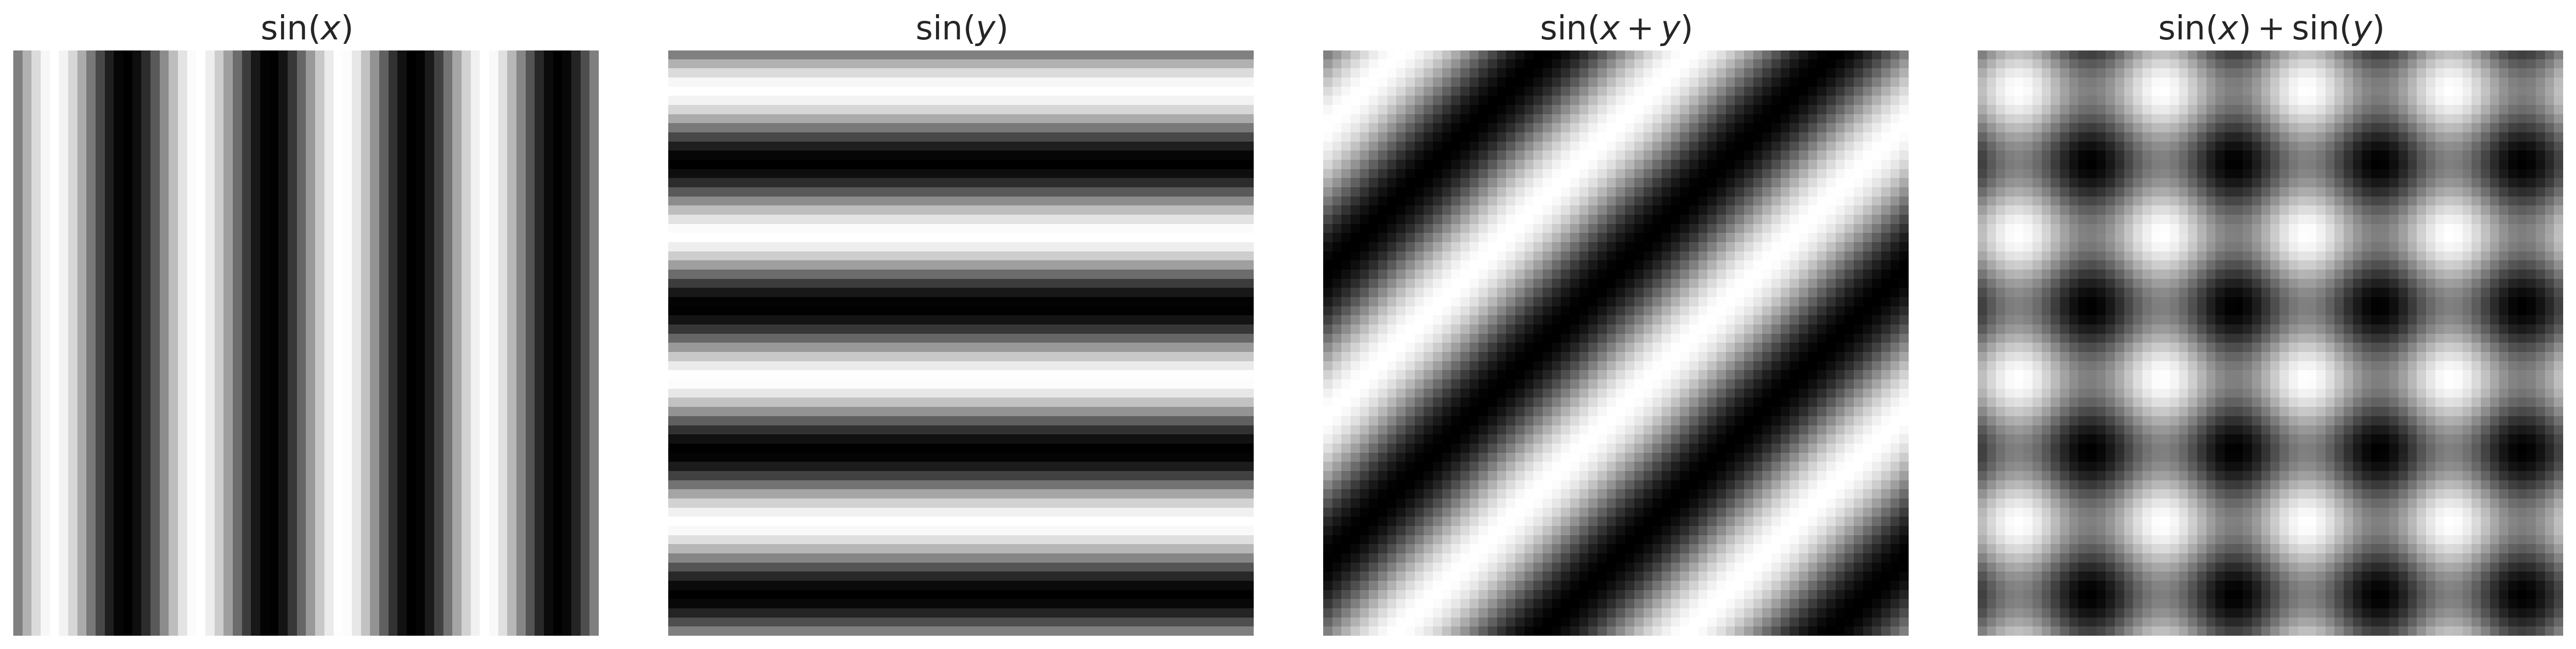
\includegraphics[width=\textwidth]{2dsin.png}
		\caption{Test 2D sinusoid patterns.}
		\label{fig:2dsin}
	\end{subfigure}
	\begin{subfigure}{\textwidth}
		\centering
		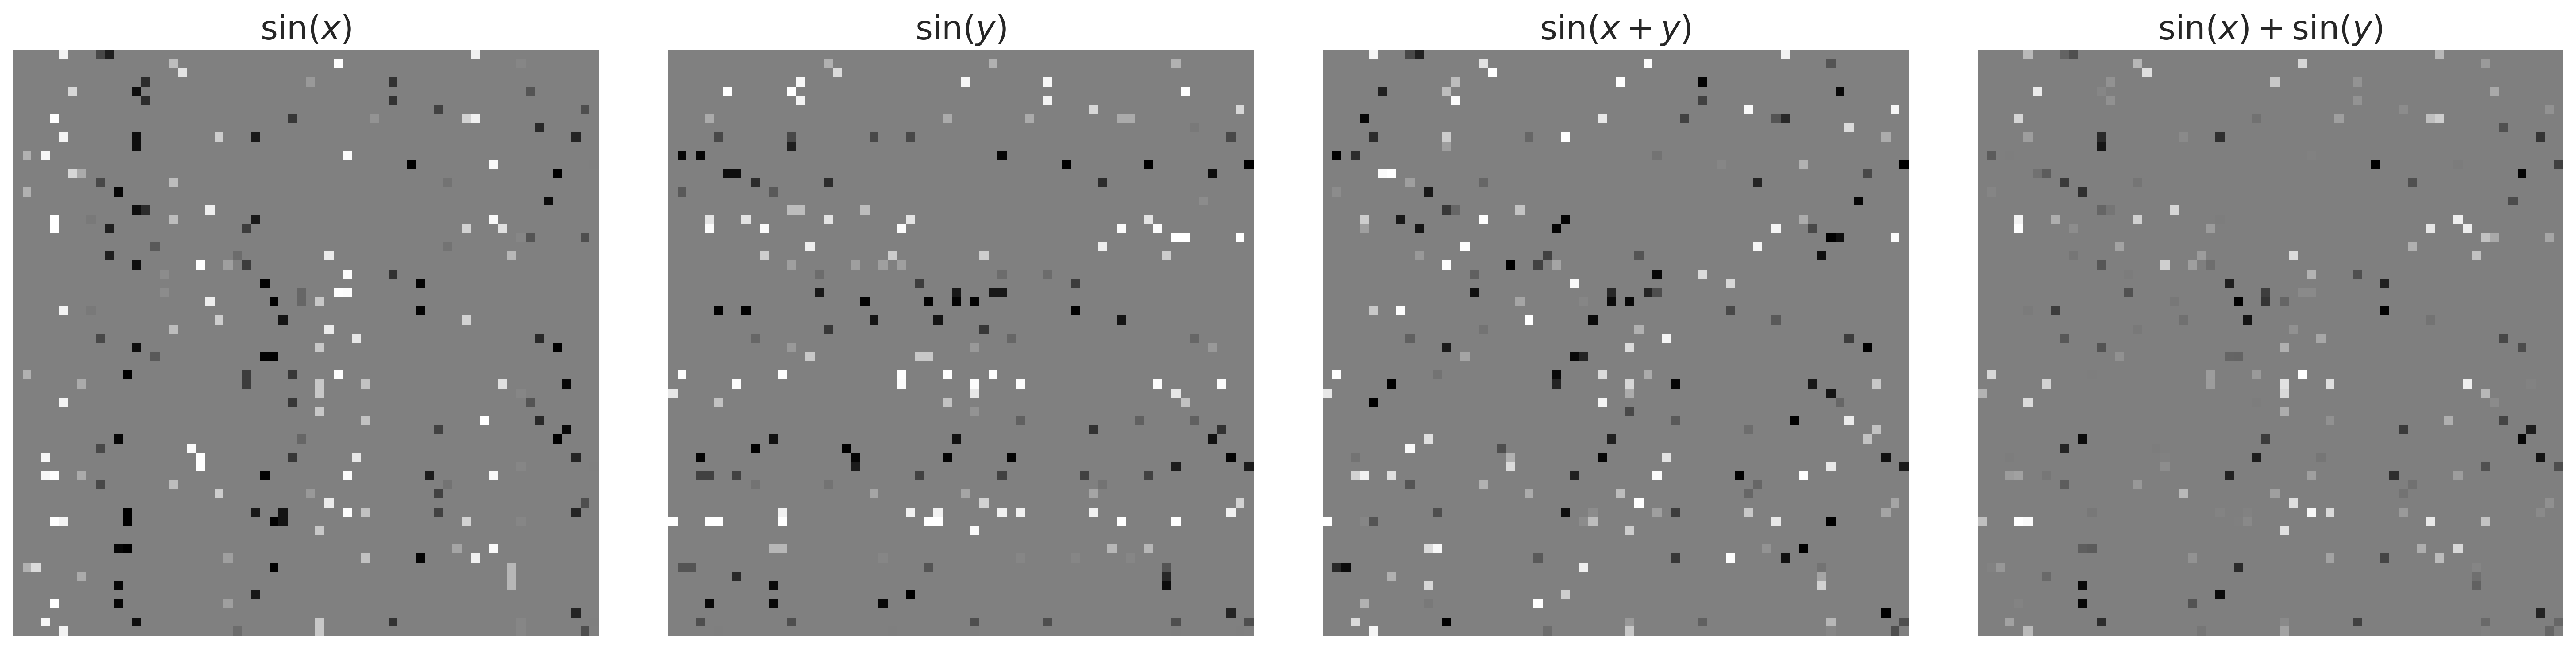
\includegraphics[width=\textwidth]{2dsin-masked.png}
		\caption{Visualization of sinusoid patterns with compression ratio of 5\%.}
		\label{fig:2dsin-masked}
	\end{subfigure}
	\begin{subfigure}{\textwidth}
		\centering
		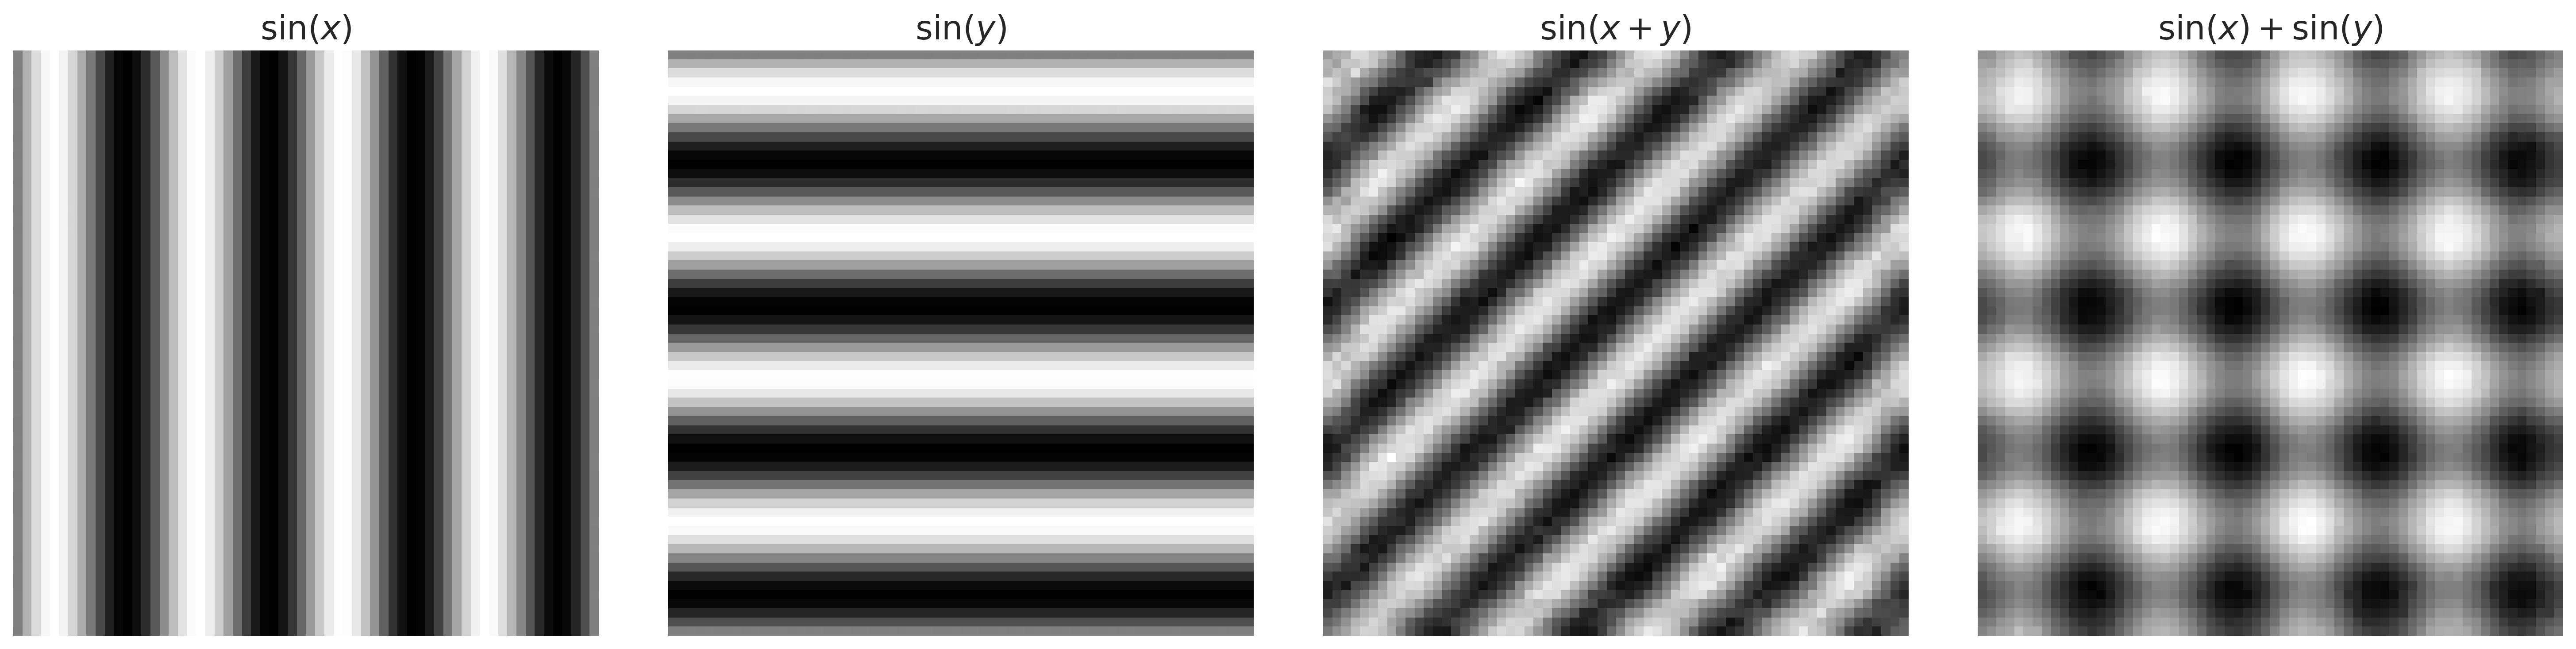
\includegraphics[width=\textwidth]{2dsin-recovered.png}
		\caption{Reconstruction from 5\% of samples.}
		\label{fig:2dsin-recovered}
	\end{subfigure}
	\caption{Test $64 \times 64$ pixel 2D sinusoid patterns corresponding to vertical sinusoids, horizontal sinusoids, diagonal sinusoids, and egg tray pattern. All frequency components are 4 Hz.}
	\label{fig:test-2dsin}
\end{figure}


\section{Image with multiple sinusoids}
\label{sec:2dmultisin}

\subsection{Pre-processing}
\label{ssec:image-multi-preprocess}
For this section, the image used is M.C. Escher's \textit{Relativity}, an example of a more complex image but consisting of dominant sinusoidal patterns that are made apparent when you zoom in. The original image has dimensions of $1600 \times 981$ pixels, for a total of 1,569,600 pixels. Following the procedure with the previous section, this would require the construction of a 1,569,600 $\times$ 1,569,600 sparsifying matrix containing $\approx 2 \times 10^{12}$ entries. Assuming that the matrix would be stored as 32-bit floating point numbers, this process alone would take up $\approx 8$ GB of memory, and it would be highly impractical to process similarly-sized images as a whole. The workaround is to split it into smaller, manageable patches. 

\subsection{Processing}
\label{ssec:image-multi-process}
For this image in particular, it was first resized to $1600 \times 976$ pixels so that it could be equally divided into a grid of $16 \times 16$, each with a dimension of $100 \times 61$ pixels. After compressively sampling each patch at 40\% compression ratio, reconstruction was performed using the Embedded Conic Solver (ECOS) of the Convex Optimization Python library (CVXPY), which recasts \eqref{eq:min-l1} as a convex problem and directly minimizes the $\ell_1$ norm \cite{ecos,cvxpy,cvxpy_rewriting} and thus, is significantly slower compared to OMP.

\subsection{Reconstruction evaluation}
\label{ssec:image-multi-error}
To quantify the reconstruction quality, the Structural Similarity Index (SSIM) \cite{Wang2004} was used. This is a perception-based model that takes into account perceptual factors such as luminance, contrast, and structure. SSIM is calculated on windows in the image, and is defined as

\begin{equation}
	\label{eq:ssim}
	\mathrm{SSIM}(\vec{x}, \bm\hat{\vec{x}}) = \frac{(2\mu_{\vec{x}}\mu_{\bm\hat{\vec{x}}} + c_1) (2\sigma_{\vec{x} \bm\hat{\vec{x}}} + c_2)}{(\mu_{\vec{x}}^2 + \mu_{\bm\hat{\vec{x}}}^2 + c_1) (\sigma_{\vec{x}}^2 + \sigma_{\bm\hat{\vec{x}}}^2 + c_2)}
\end{equation}

\noindent where $\vec{x}, \bm\hat{\vec{x}}$ are the original and reconstructed signals, respectively, $\mu$ are the image means, $\sigma$ are the image standard deviations, and $c$ are constants to stabilize division with a small denominator. SSIM values of 0.8 and above are considered acceptable.

After stitching all patches at the end, the reconstructed image is shown in Fig.~\ref{fig:relativity-recovered}. Evaluation of SSIM yields a value of 0.88, way above the acceptable threshold. Selected patches with the aforementioned dominant patterns are shown with their reconstructed counterparts in Fig.~\ref{fig:relativity-dominant-slices}, corresponding to patches dominated by horizontal sinusoids, vertical sinusoids, diagonal sinusoids, multiple sinusoids, and patches with no dominant pattern.

We can observe that at this compression rate, the patches with a single apparent sinusoidal pattern (Figs.~\ref{fig:relativity-vert40}-\ref{fig:relativity-diag40}) are successfully recovered, with some noise present especially for the patch with a dominant diagonal pattern (similar to the previous section). The patch with multiple sinusoid patterns (Fig.~\ref{fig:relativity-mult40}), although still recognizable, is laden with a lot of noise. Lastly, the patch with no apparent pattern (Fig.~\ref{fig:relativity-high40}) is barely recognizable, except for the portions where a dominant sinusoidal pattern is partially present in the frame.

From this, the following information can be gleaned. First, reconstruction performs better on smaller patches, and when the patch in question contains as few frequency components as possible (such is the case with the patches with only one dominant pattern). Second, the patch with no dominant pattern---upon closer visual inspection---can be classified as being successfully recovered; however, the reconstruction noise is almost at the same level as the signal itself, which makes them indistinguishable. This can be attributed to the fact that the patches with no apparent dominant pattern are actually composed of a superposition of sinusoids residing primarily in the high-frequency region of $k$-space. Since the sampling points are uniformly distributed throughout the spatial domain, so are they in the frequency domain. Thus, the information in the high-frequency region is not sufficiently captured, and a higher compression ratio is required to be able to better recover these high-frequency regions. Another solution would be, as mentioned earlier, to make the patches smaller so that lesser frequencies are captured in one patch.

\begin{figure}[htb]
	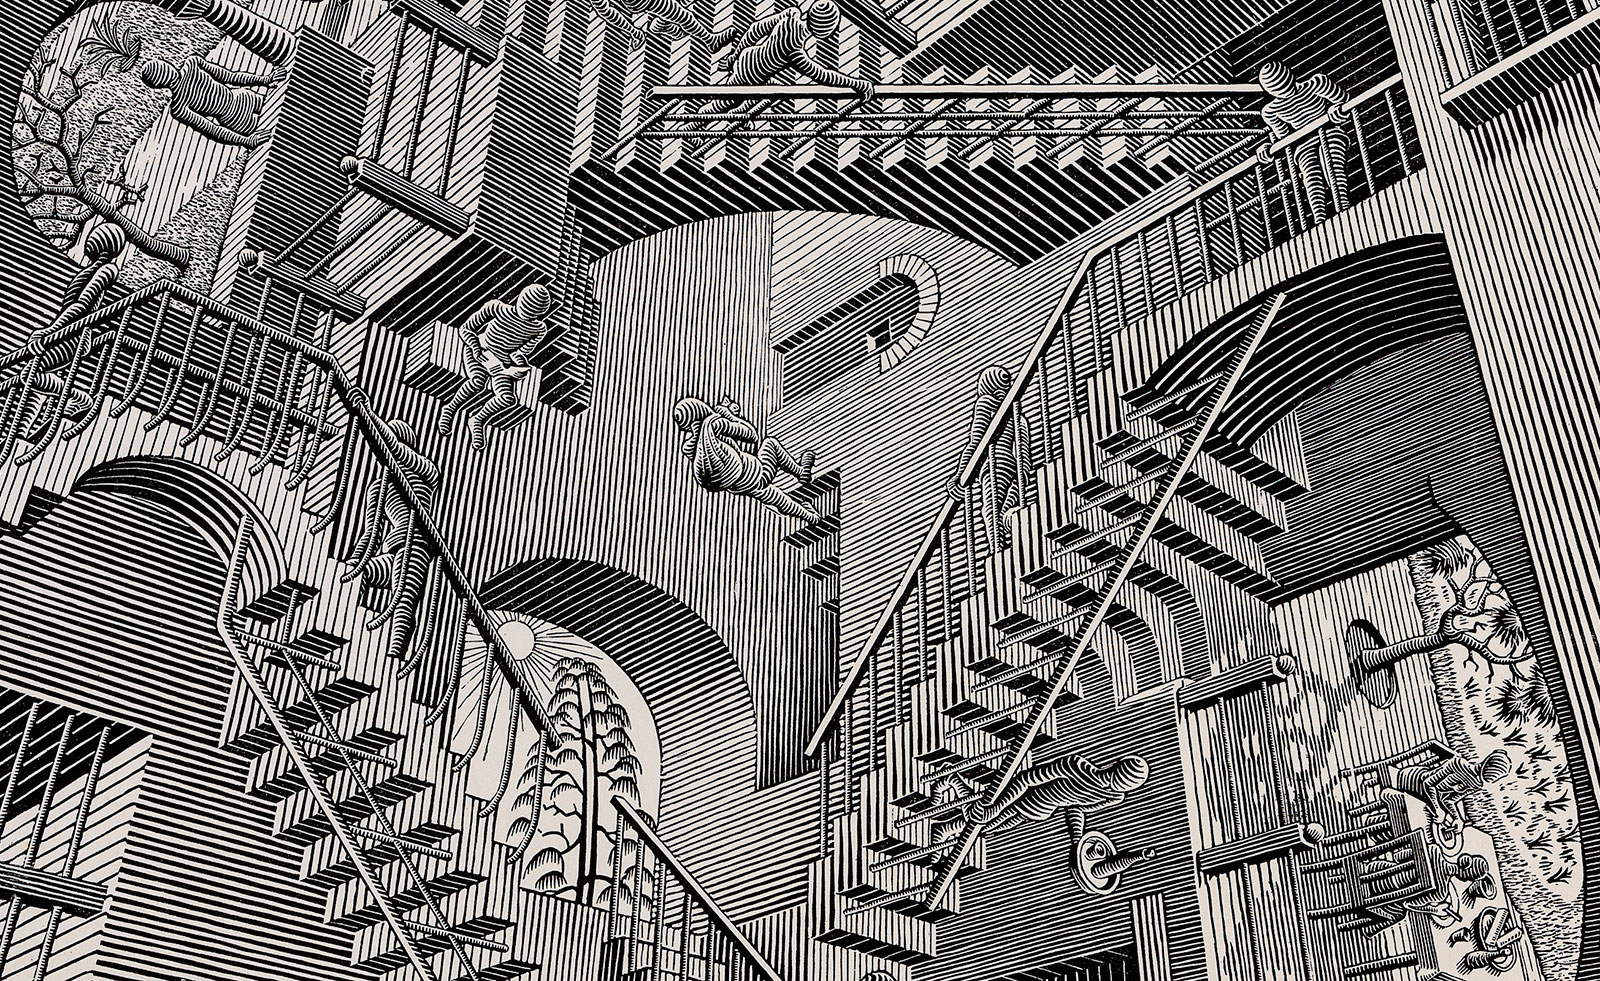
\includegraphics[width=\textwidth]{relativity.jpg}
	\caption{\textit{Relativity} by M.C. Escher, a complex image consisting of various sinusoidal patterns.}
	\label{fig:relativity}
\end{figure}

\begin{figure}[htb]
	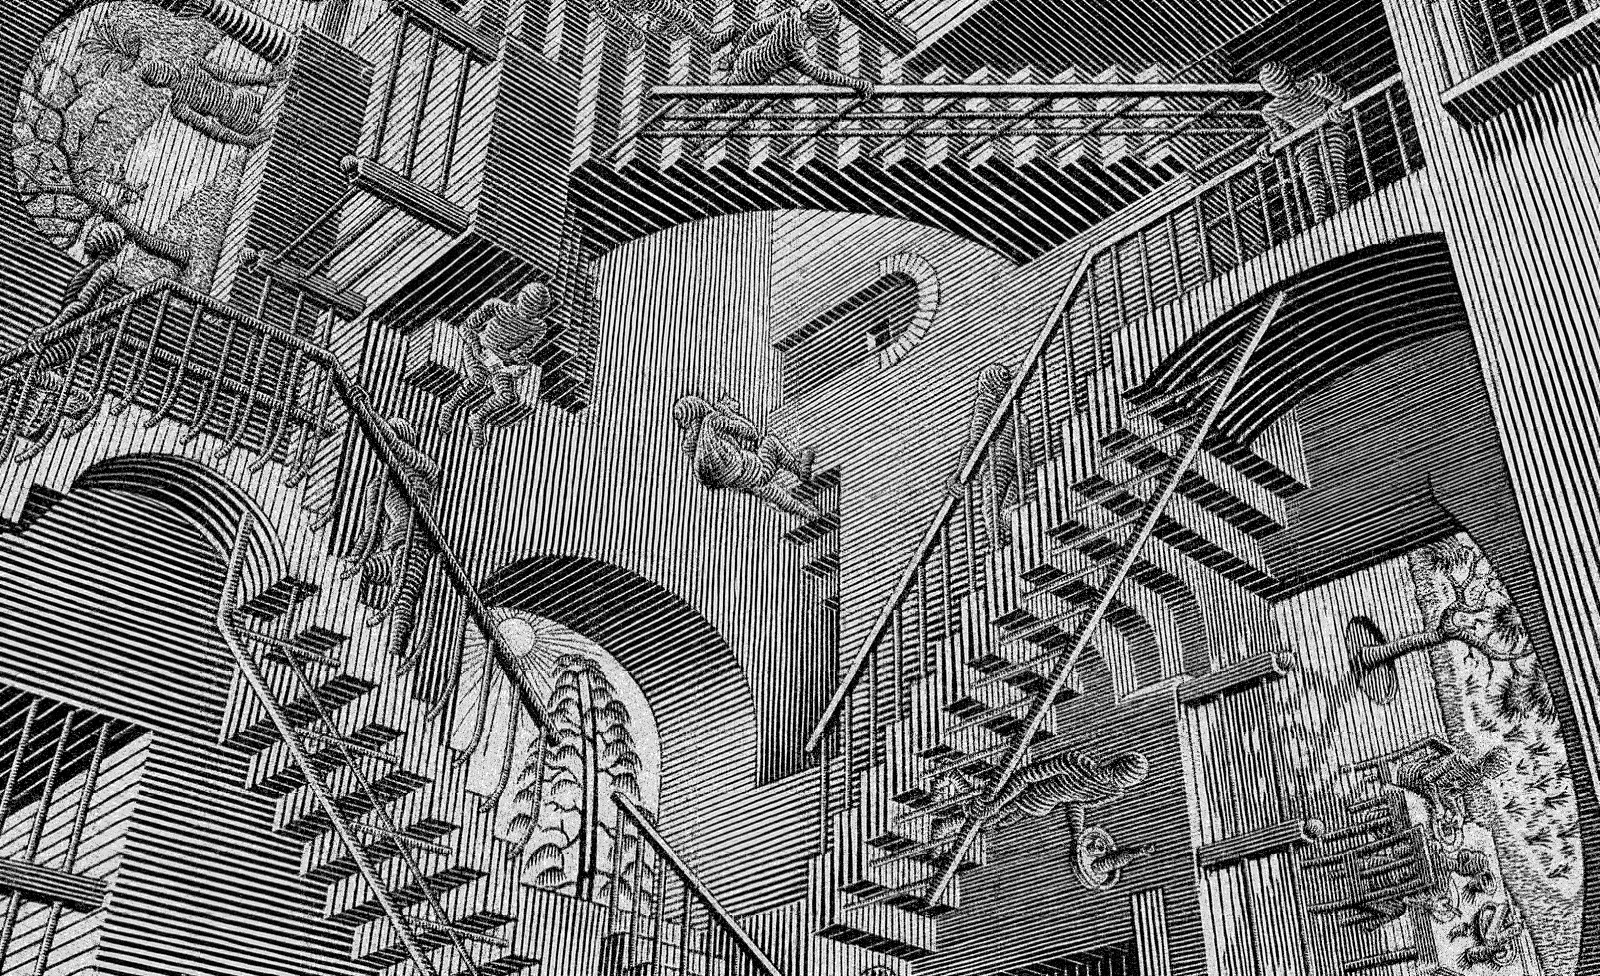
\includegraphics[width=\textwidth]{relativity-recovered.png}
	\caption{Reconstructed \textit{Relativity} from 50\% of samples from each patch.}
	\label{fig:relativity-recovered}
\end{figure}

\begin{figure}[htb]
	\centering
	\begin{subfigure}{\textwidth}
		\centering
		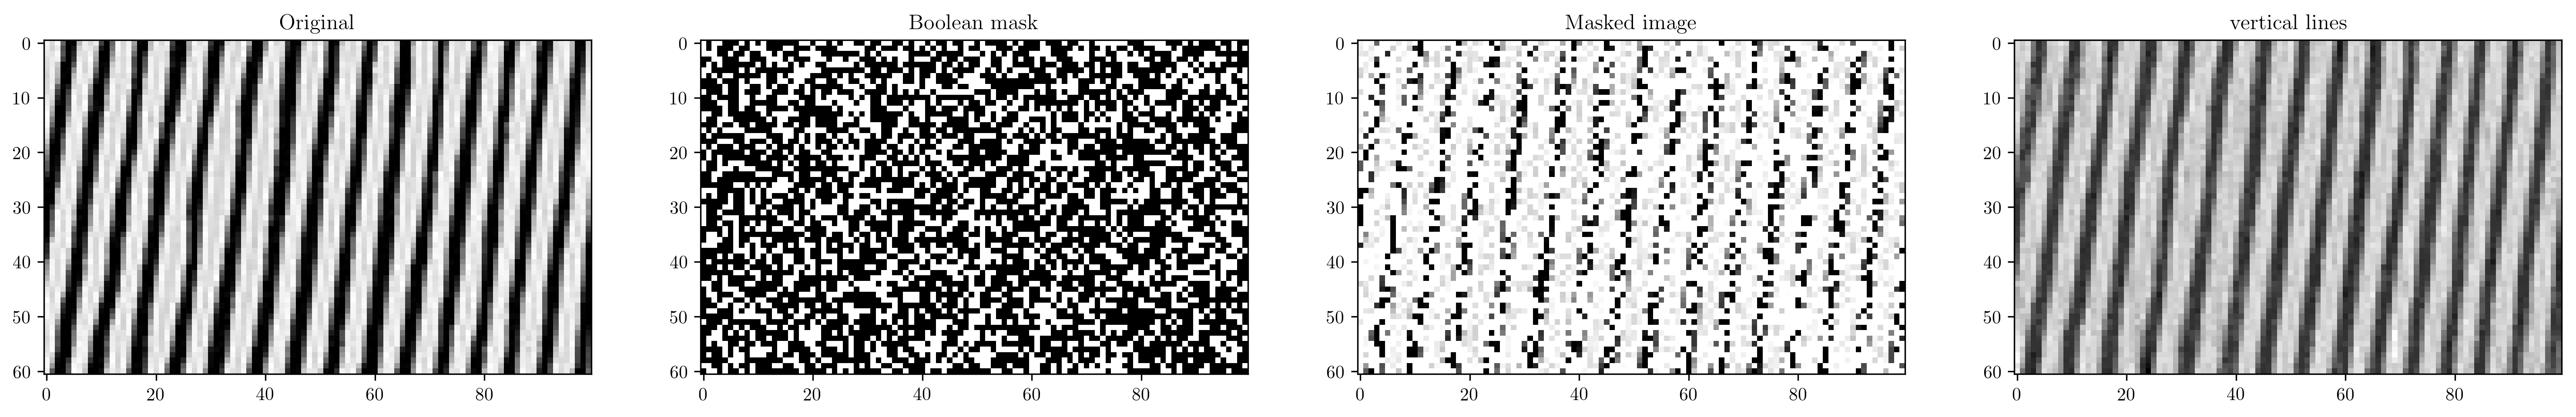
\includegraphics[width=\textwidth]{relativity-vert40.png}
		\caption{Dominant vertical}
		\label{fig:relativity-vert40}
	\end{subfigure}
	\begin{subfigure}{\textwidth}
		\centering
		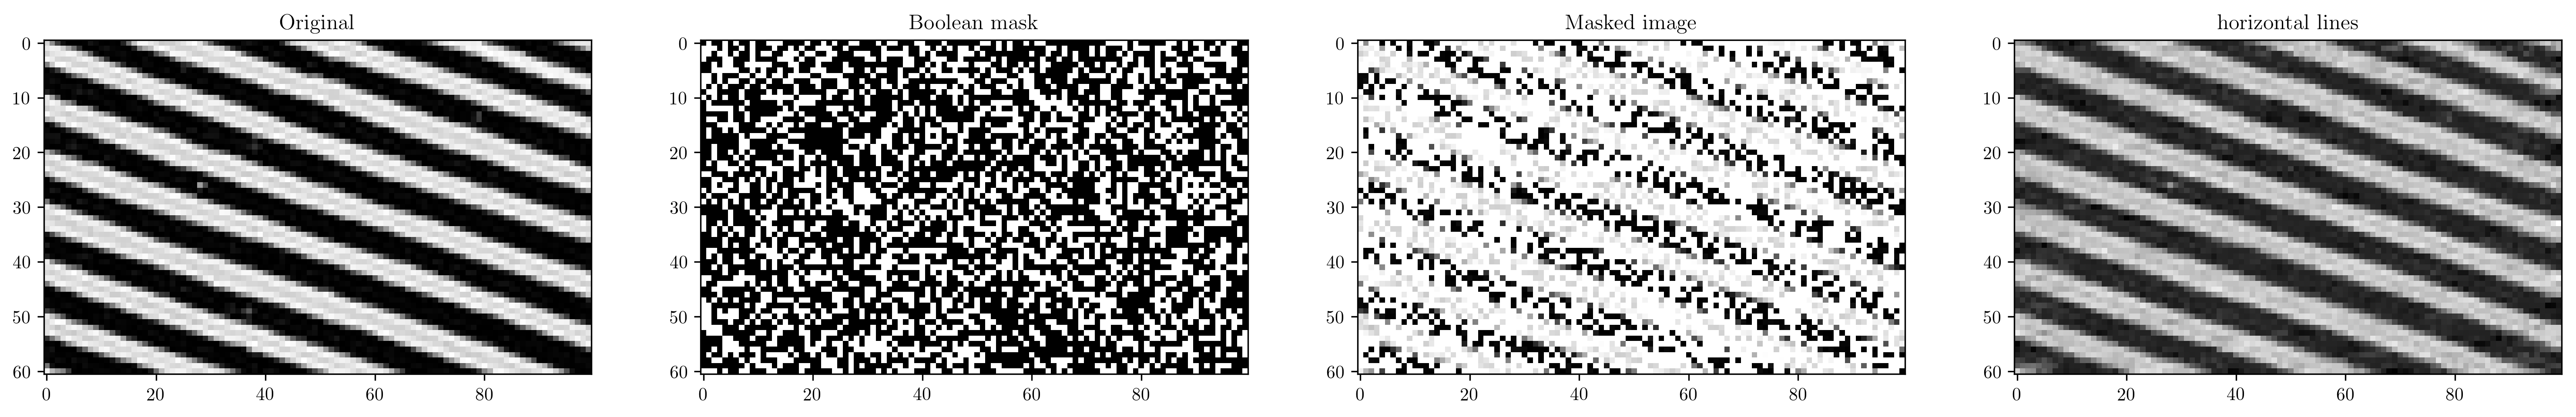
\includegraphics[width=\textwidth]{relativity-horiz40.png}
		\caption{Dominant horizontal}
		\label{fig:relativity-horiz40}
	\end{subfigure}
	\begin{subfigure}{\textwidth}
		\centering
		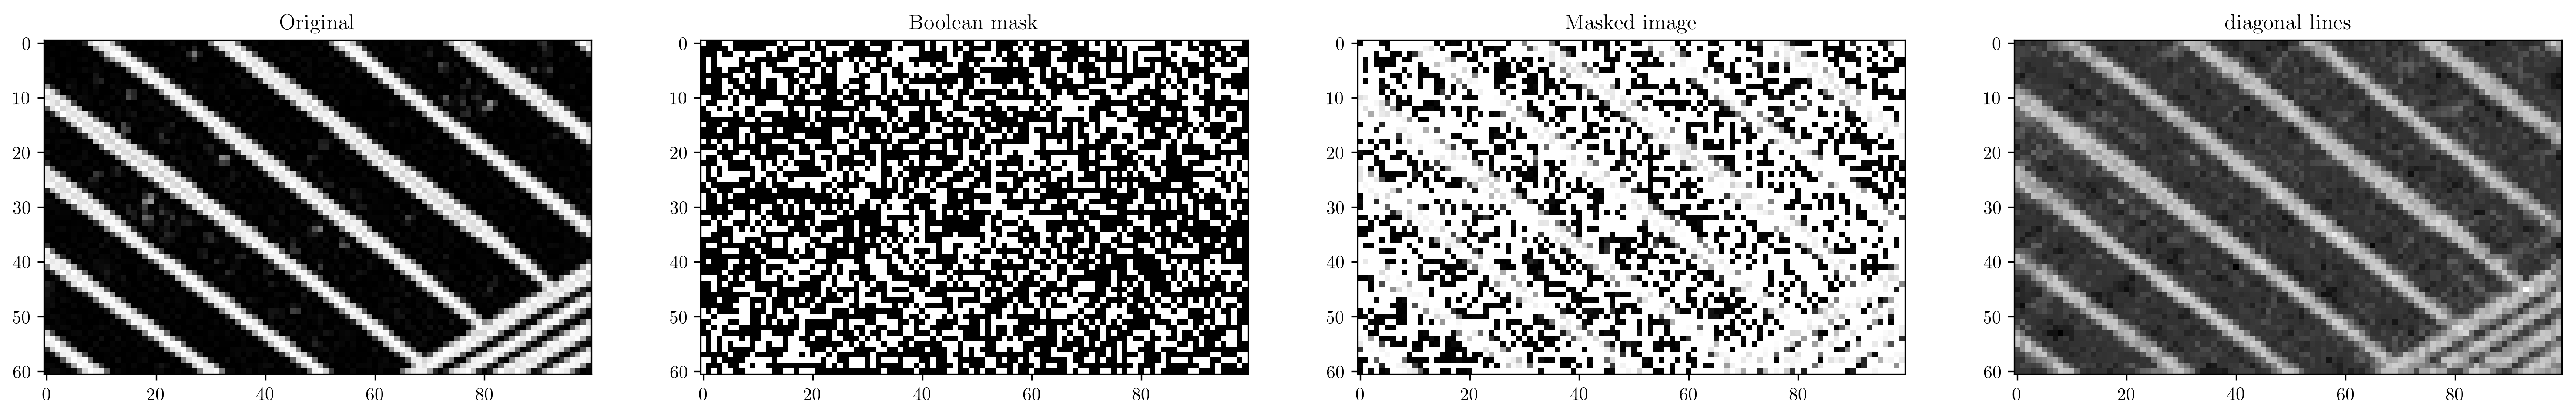
\includegraphics[width=\textwidth]{relativity-diag40.png}
		\caption{Dominant diagonal}
		\label{fig:relativity-diag40}
	\end{subfigure}
	\begin{subfigure}{\textwidth}
		\centering
		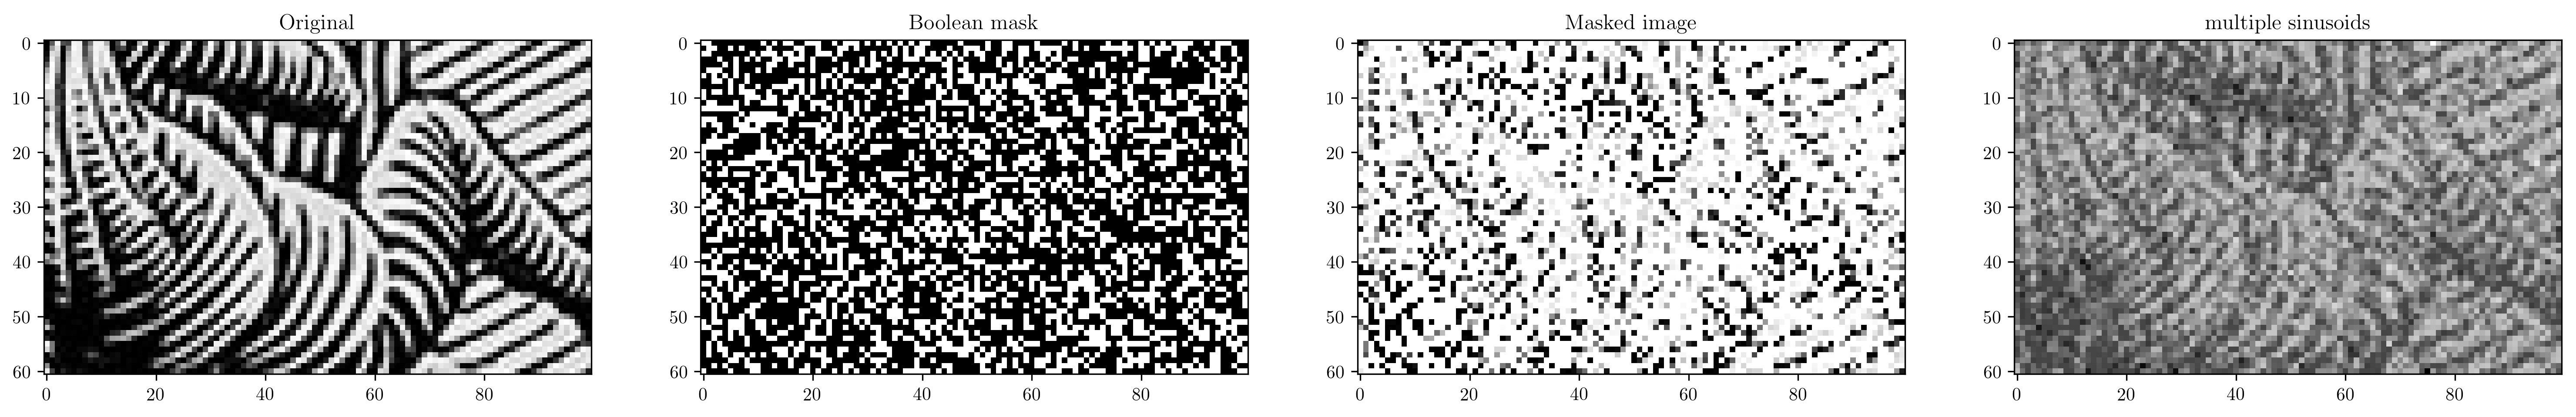
\includegraphics[width=\textwidth]{relativity-mult40.png}
		\caption{Multiple dominant sinusoids}
		\label{fig:relativity-mult40}
	\end{subfigure}
	\begin{subfigure}{\textwidth}
		\centering
		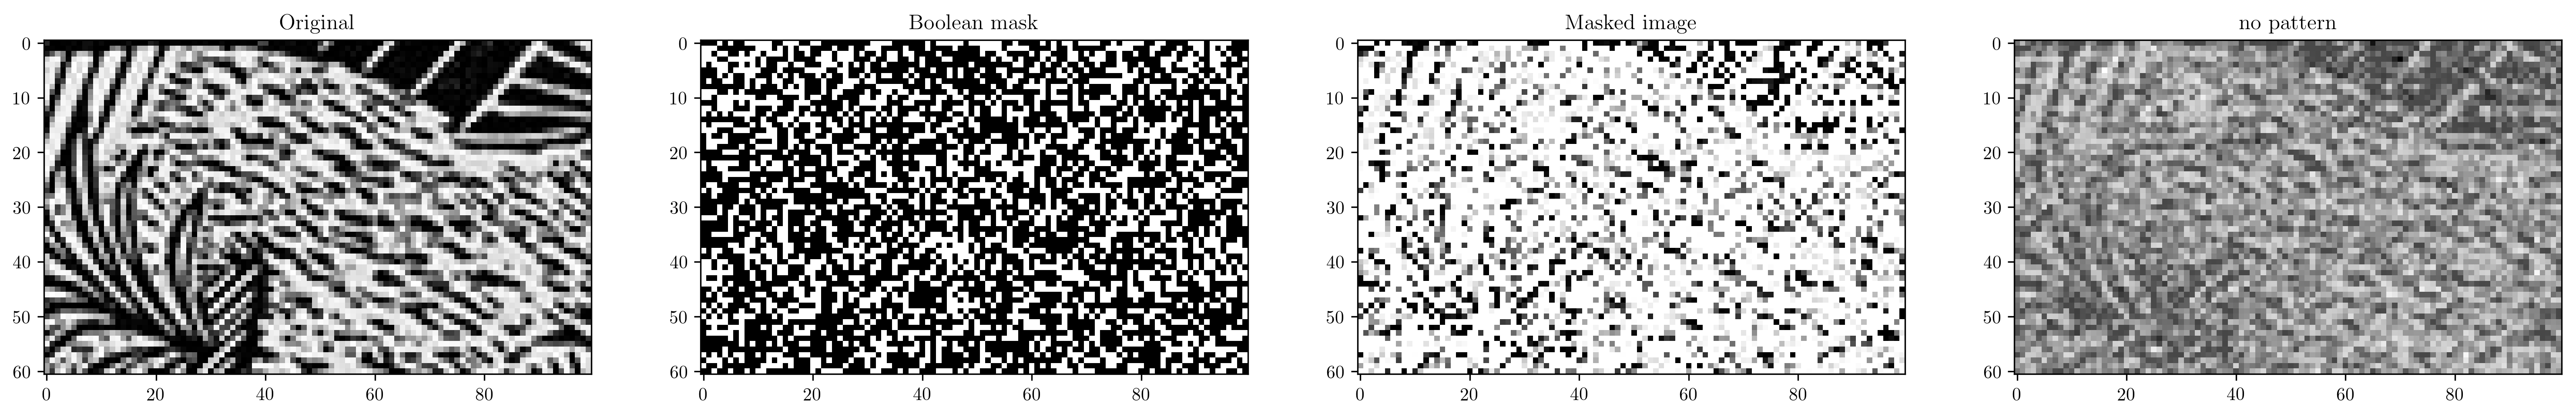
\includegraphics[width=\textwidth]{relativity-high40.png}
		\caption{No dominant pattern}
		\label{fig:relativity-high40}
	\end{subfigure}
	\caption{Extracted and reconstructed patches from \textit{Relativity} using 40\% of samples.}
	\label{fig:relativity-dominant-slices}
\end{figure}


\section{Simultaneous compression \& encryption}
Because of the way compressively sampled images are coded with the sensing matrix, the use of CS as an encryption algorithm arises naturally. Consider the logistic map

\begin{equation}\label{eq:logistic-map}
	x_{n+1} = r x_n \qty(1 - x_n)
\end{equation}

\noindent which is often used as an archetypal example of deterministic chaotic behavior for values of $r \in [3.57, 4)$. In this regime, the sequences produced by varying the initial parameter $x_0$ rapidly diverge from each other. Thus, this can become an encryption system by treating the parameters $r$ and $x_0$ as an encryption key set, and \eqref{eq:logistic-map} as the hash function. One key set is then needed for each signal dimension. Thus, two key sets are needed for grayscale image applications (six, in the case of an RGB image and a unique key set for each color channel). 

\subsection{Methodology}
\label{ssec:image-encrypt-metho}
The construction of the sensing matrix $\bm\Phi$ differs from the general workflow, and is as follows:

\begin{enumerate}
	\item From \eqref{eq:logistic-map}, generate a sequence of length $2m$ with the initial key pair $r_1$ and $x_{01}$. Discard the first $n$ elements to avoid the transient response and store the latter $n$ elements as a sequence $\vec{s}$.
	\item Explicitly generate the index sequence of $\vec{s}$ and store it as sequence $\vec{p} = \qty[0, 1, ..., m-1]$.
	\item Sort $\vec{p}$ according to ascending values of $\vec{s}$.
	\item Generate the first sensing matrix $\bm\Phi_1$ by extracting and stacking rows of a Hadamard matrix $\vec{H}$ of order $N$ indexed by the first $m$ elements of $\vec{p}$, i.e.,
	\begin{equation}\label{eq:construct-hadamard}
		\bm\Phi_1 = \mqty[
			\vec{H}_{p_1} & \vec{H}_{p_2} & \cdots & \vec{H}_{p_m}
		]^\top
	\end{equation}
	\noindent where $\vec{H}_{p_i}$ denotes the $p_i$th row vector of $\vec{H}$.
	\item Any other sensing matrices can be constructed in the same way.
\end{enumerate}

The usage of a Hadamard matrix implies that the image must first be reshaped to have dimensions that are integer multiples of 4. The original image is first reshaped to $256 \times 256$ pixels, and is sparsified by transforming it to the DCT domain. The desired compressed dimension is set to $m = 192$, corresponding to a compression ratio of 75\%, and the keys are set to values of $r_1 = r_2 = 3.99$, $x_{01} = 0.11$, and $x_{02} = 0.24$.

\subsection{Results \& discussion}
\label{ssec:image-encrypt-rnd}
Figure~\ref{fig:encryption} shows the application of this to the Lena test image. Visual inspection of the encrypted representation shows horizontal and vertical bands distributed throughout the representation space, and is indicative that a simple inverse Fourier transform will not recover any meaningful information. Assuming that the receiver knows the encryption scheme, recovery of the original message is successful if the same keys $r_1, r_2, x_{01}, x_{02}$ as the encryption stage are used, which will allow the receiver to construct the exact same sensing matrices $\bm\Phi_1, \bm\Phi_2$ and perform the inverse operation on the encrypted message. In the decrypted image, encryption artifacts can be observed, as indicated by some visible banding, but is nonetheless recognizable; evaluation of the MSE and SSIM yields values of 0.02 and 0.82, respectively.

\begin{figure}[htb]
	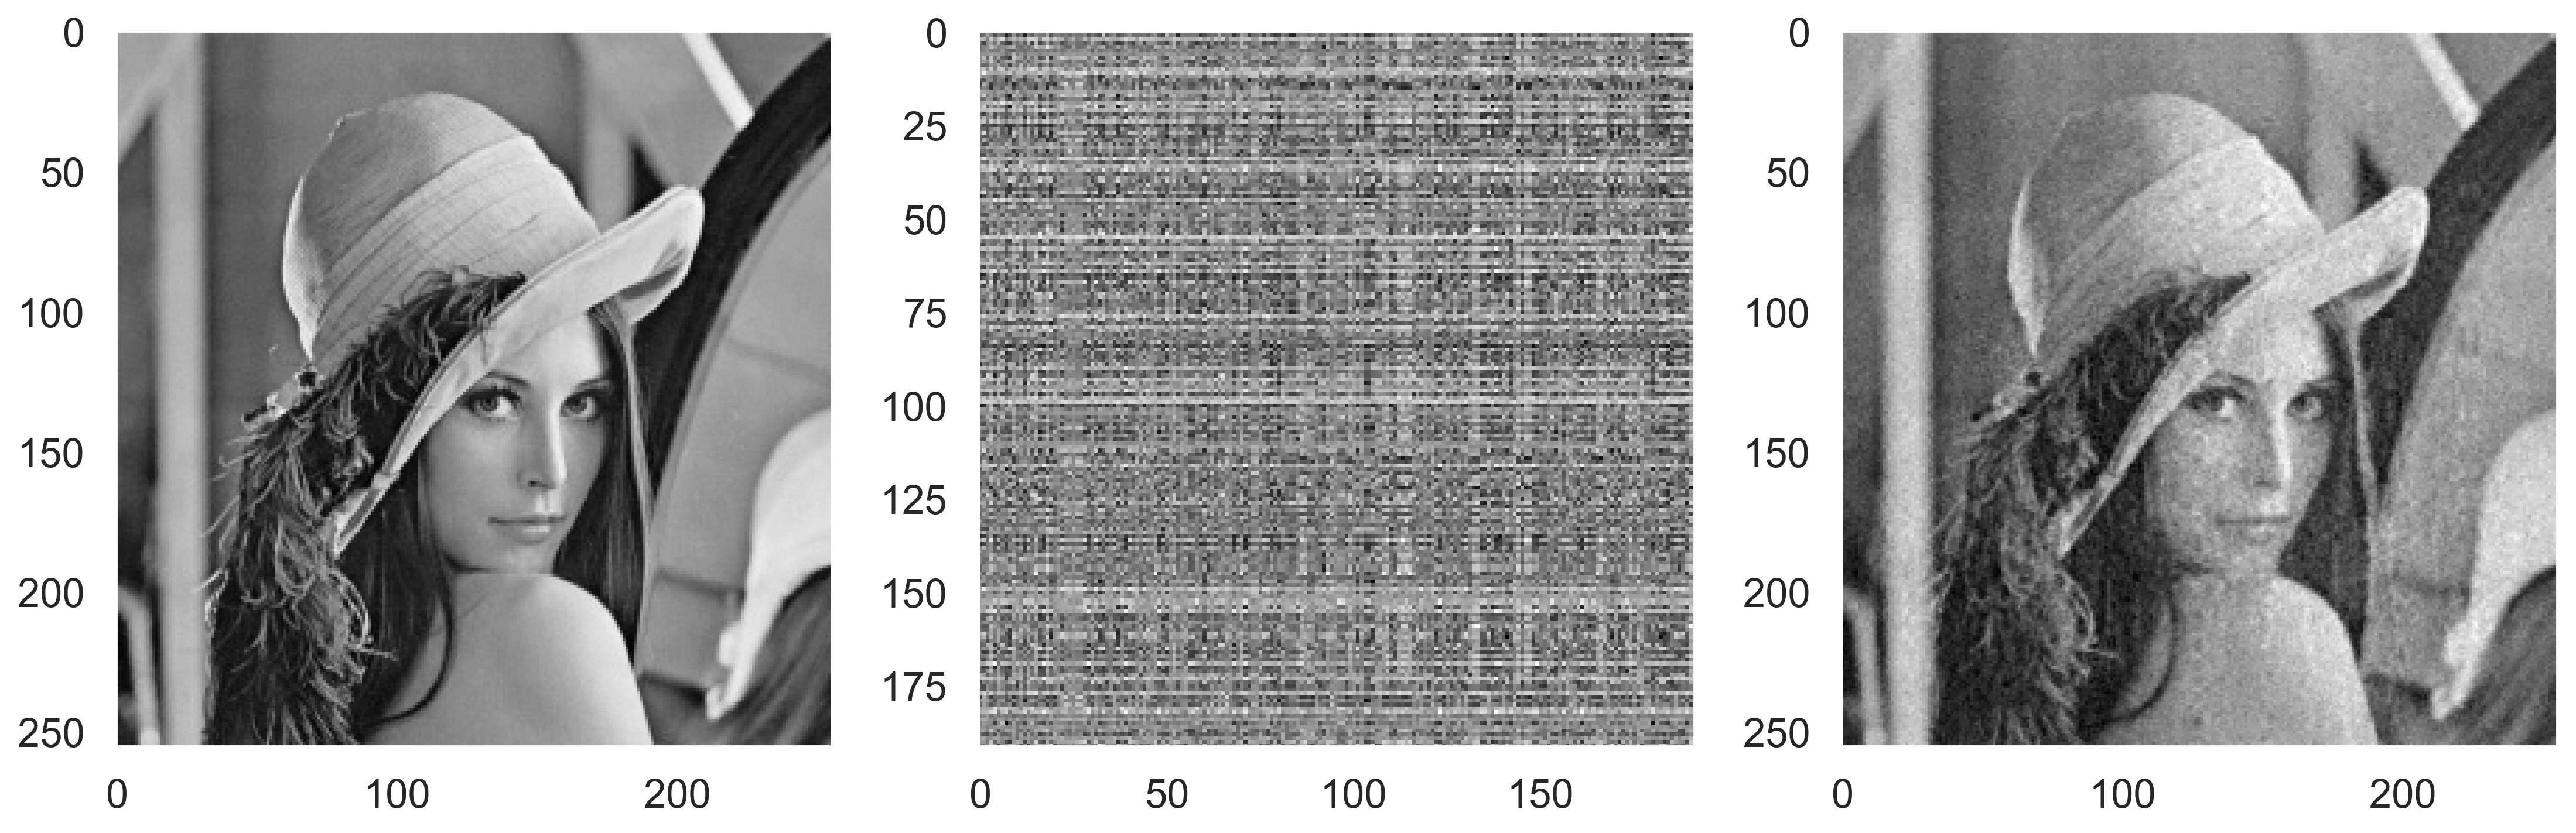
\includegraphics[width=\textwidth]{encryption.png}
	\caption{Simultaneous compression and encryption achieved with compressive sensing: original image (left), encrypted image (middle), and decrypted/reconstructed image (right).}
	\label{fig:encryption}
\end{figure}

\subsection{Correlation analysis}
\label{ssec:image-encrypt-correlation}
Correlation is a statistical measure of obtaining useful information from a given signal by analyzing adjacent pixels. The correlation coefficients can be obtained by

\begin{equation}
	\label{eq:correlation-coeff}
	C = \frac{\sum_{i=1}^N (x_i - \ev{\vec{x}}) (y_i - \ev{\vec{y}}}{\sqrt{\sum_{i=1}^N (x_i - \ev{\vec{x}})^2 \sum_{i=1}^N (y_i - \ev{\vec{y}})^2}}
\end{equation}

\noindent where $\vec{x}$ and $\vec{y}$ are the original and encrypted signals, respectively. For the purposes of encryption, a correlation coefficient closer to 0 is better. Table~\ref{tab:correlation} shows the computed correlations for the original and encrypted Lena images in the horizontal, vertical, and diagonal directions. The correlation of the encrypted signal is much lower than that of the original, which means that a potential attacker cannot gain any useful information by employing statistical analyses.

\begin{table}
	\centering
	\caption{Correlation coefficients of test Lena image.}
	\label{tab:correlation}
	\begin{tabular}{rrrr}
		\toprule
		 & horizontal & vertical & diagonal \\
		 \midrule
		 original & 0.94 & 0.97 & 0.91 \\
		 encrypted & 0.42 & 0.02 & $-0.05$ \\
		 \bottomrule
	\end{tabular}
\end{table}


\subsection{Key sensitivity analysis}
\label{ssec:image-encrypt-keysensitivity}
With the knowledge that the hash function $\eqref{eq:logistic-map}$ is chaotic, the sensitivity of the encryption system to the keys can be tested by perturbing the initial keys with small values. Figure~\ref{fig:wrong-decryption} shows the decryption results when all the correct keys are used, except for $x_{01}$, which is perturbed by a tiny value $\approx 10^{-15}$ (third image), and similarly when the correct $x_{01}$ is used but $x_{02}$ is perturbed by the same amount (last image).

\begin{figure}[htb]
	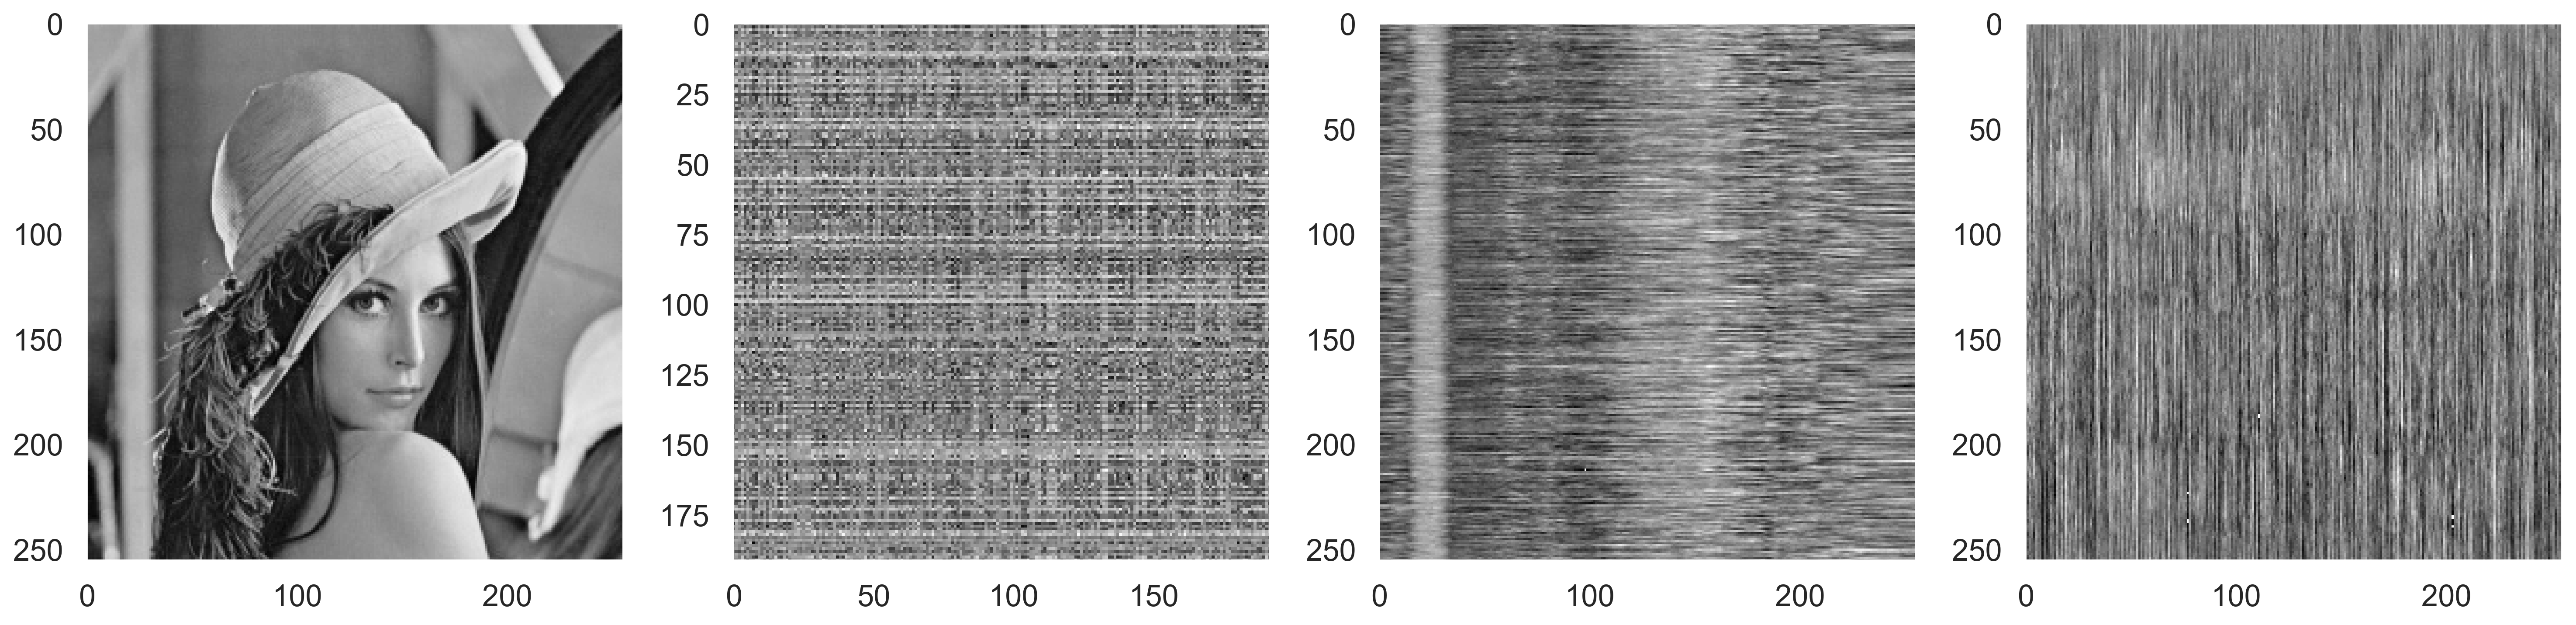
\includegraphics[width=\textwidth]{wrong_decrypt.png}
	\caption{Test image Lena (first) with the encrypted representation (second), the decryption result when the correct keys are used but $x_{01}$ is perturbed by a value of $10^{-15}$ (third), and the decryption result when the correct keys are used but $x_{02}$ is perturbed by a value of $10^{-15}$.}
	\label{fig:wrong-decryption}
\end{figure}

Additionally, Fig.~\ref{fig:perturb-mse} shows the MSE curves evaluated by varying values of the perturbation $\Delta x_{01}$ and $\Delta x_{02}$. The MSE generally oscillates at some high value for perturbations on the degree of $10^{-15}$, and exhibits a sharp dip when the MSE is evaluated for the correct keys ($\Delta x_0 = 0$). This shows that brute force attacks are intractable against this kind of encryption system.

\begin{figure}[htb]
	\centering
	\begin{subfigure}{0.49\textwidth}
		\centering
		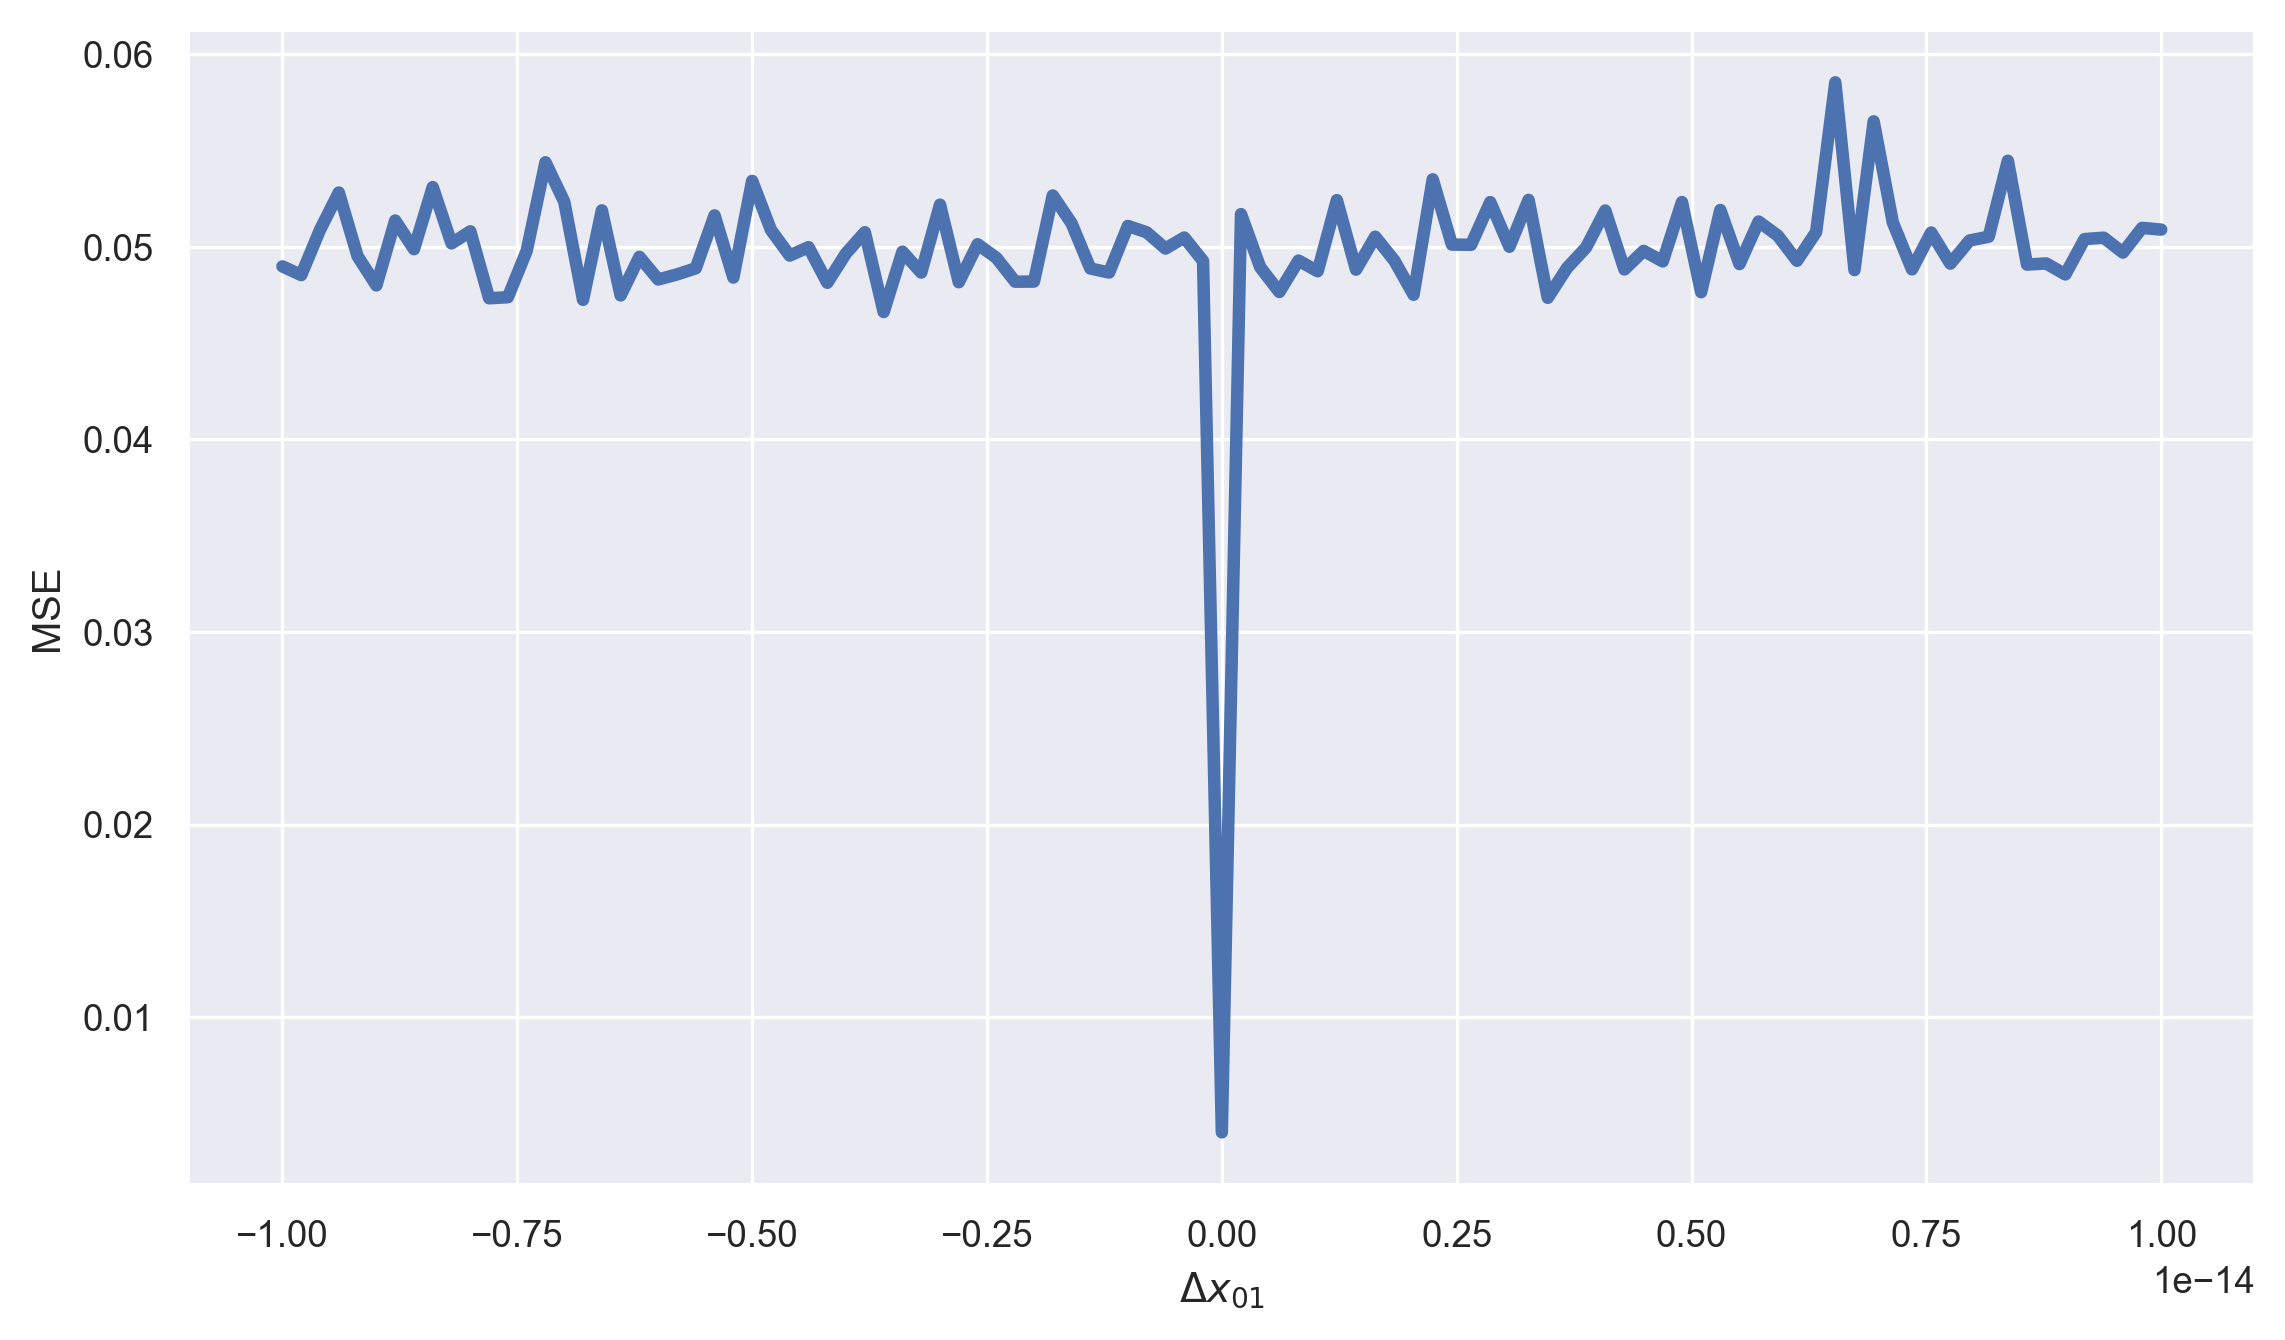
\includegraphics[width=\textwidth]{mse-x01.png}
		\caption{Perturbation of $\Delta x_{01}$}
		\label{fig:perturb-mse-x01}
	\end{subfigure} 
	\begin{subfigure}{0.49\textwidth}
		\centering
		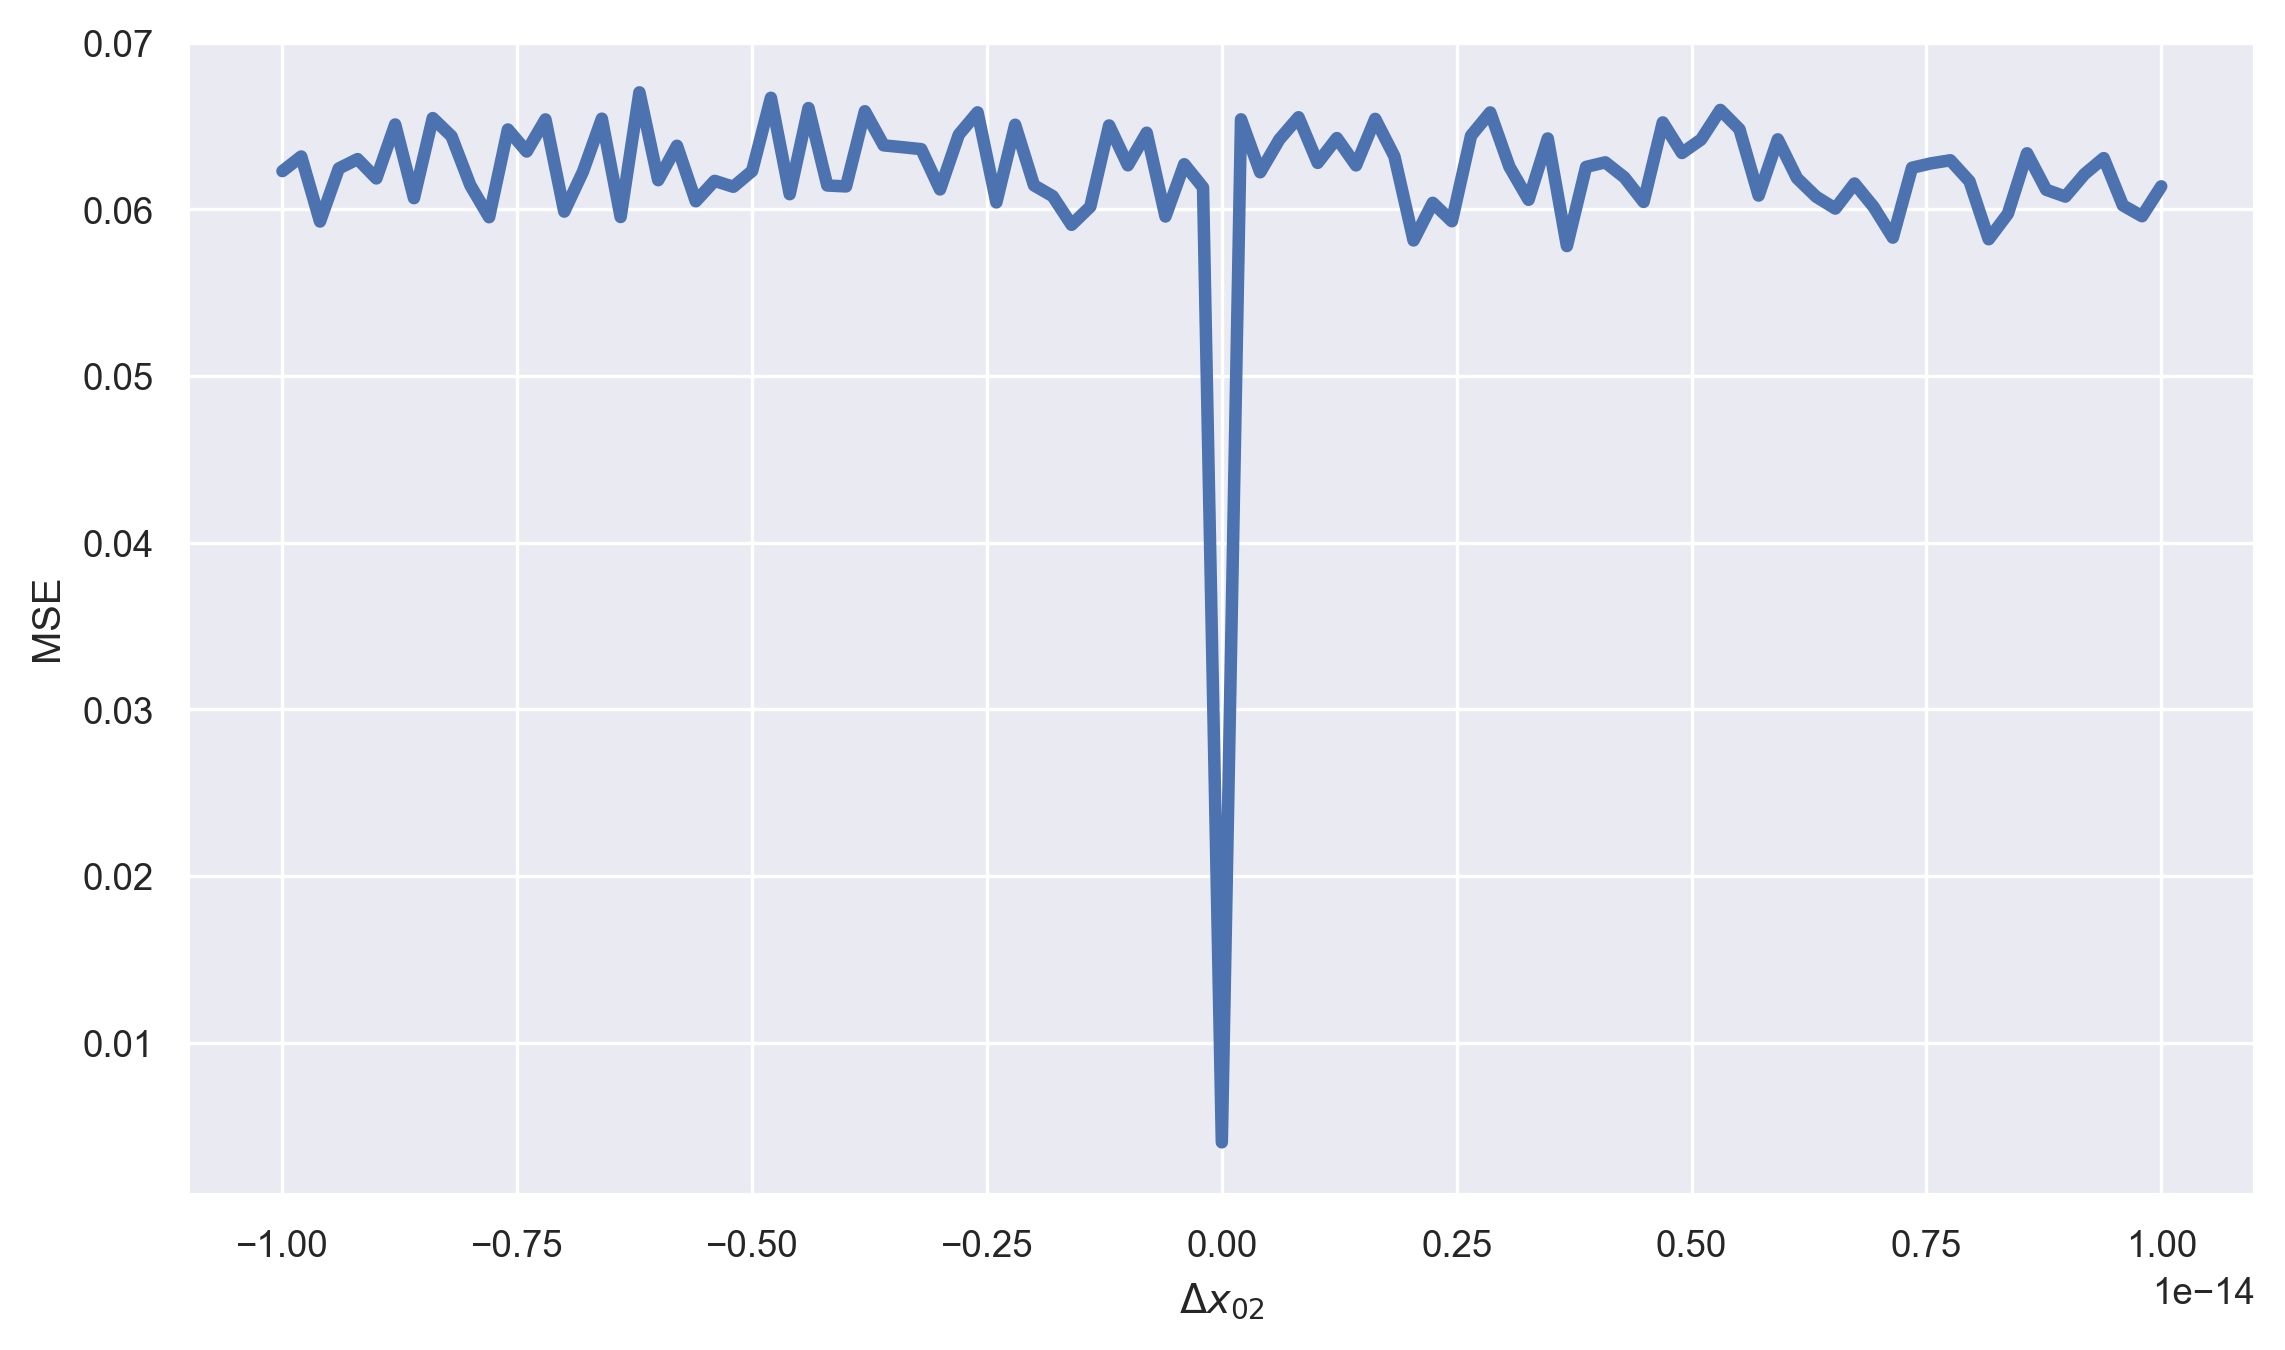
\includegraphics[width=\textwidth]{mse-x02.png}
		\caption{Perturbation of $\Delta x_{02}$}
		\label{fig:perturb-mse-x02}
	\end{subfigure}
	\caption{MSE curves resulting from evaluation of reconstruction error for tiny perturbations in the initial values $\Delta x_{01}$ and $\Delta x_{02}$.}
	\label{fig:perturb-mse}
\end{figure}